\documentclass[sigconf]{acmart}

\usepackage{booktabs}
\usepackage{graphicx}
\usepackage{amsmath}
\usepackage{subcaption}

\setcopyright{none}
\acmConference[ICAIL '25]{International Conference on Artificial Intelligence and Law}{2025}{India}

\title{Multi-Agent Judicial Decision Support: Prioritization, Semantic Retrieval, and Explainability Under the IPC-to-BNS Statutory Transition}

\author{Akshaya R}
\affiliation{%
  \institution{Department of Computer Science and Engineering}
  \country{India}
}

\begin{abstract}
The Indian judicial system faces a pendency crisis exceeding 50 million cases, exacerbated by the historic transition from the Indian Penal Code (IPC, 1860) to the Bharatiya Nyaya Sanhita (BNS, 2023). We present a judicial decision-support prototype for docket triage, case summarization, cross-regime precedent retrieval, and explainable prioritization. Priority labels are generated from a predefined scoring formula and used to train an XGBoost approximation; they are not lawyer-adjudicated urgency labels. A LangGraph workflow with a conditional LLM deliberation step reviews priority signals and generates an illustrative triage draft for human review. In an illustrative 180-day courtroom scenario analysis with 30 paired seeds and three assumed workload levels, both the composite priority policy and a direct threat-first baseline reduced simulated scenario-urgent waits relative to FIFO; the composite did not outperform threat-first on urgent-tail waits. Urgency labels, arrivals, and service targets are scenario assumptions; arrivals are bootstrap samples of existing case profiles, not observed filings, and urgency has not yet been lawyer-validated. In cross-regime retrieval, BM25, Legal-BERT, and rank fusion are compared by ranking overlap; no relevance judgments are available. Model attribution results describe how the model reproduces the constructed labels and do not establish agreement with legal experts.
\end{abstract}

\keywords{Judicial AI, Case Prioritization, Legal-BERT, Explainable AI, Multi-Agent Systems, LangGraph, BNS Translation}

\maketitle

\section{Introduction}
Court backlog remains one of the most pressing governance challenges in modern democracies. In India alone, over 50 million cases remain pending across the Supreme Court, High Courts, and subordinate judiciary. Urgent matters—such as bail petitions, habeas corpus motions, and capital offences—routinely compete for court listing time with decades-old procedural civil disputes.

This backlog has been further compounded by the introduction of the \textit{Bharatiya Nyaya Sanhita} (BNS) in July 2024, replacing the 164-year-old \textit{Indian Penal Code} (IPC). While new filings cite modern BNS sections, 75 years of binding Supreme Court precedents are indexed under IPC sections. Without an automated statutory bridge, keyword-based search fails to retrieve relevant historical authorities.

To address these challenges, we introduce an integrated, multi-agent judicial decision support system featuring:
\begin{enumerate}
    \item \textbf{Cross-Regime Statutory Bridge}: A bidirectional mapping between 494 IPC and BNS sections with punishment-grounded severity indexing.
    \item \textbf{Intelligent Prioritization Agent}: A hybrid rule-and-ML scheduler optimizing court throughput based on statutory offence gravity, personal liberty, societal impact, and backlog age.
    \item \textbf{LangGraph Reconciliation Agent}: A workflow with a conditional LLM deliberation step that flags priority, explainability, and demographic-language review signals.
    \item \textbf{Illustrative Courtroom Simulation}: A paired-seed sensitivity analysis comparing scheduling policies under three assumed workload levels.
\end{enumerate}

\section{Related Work}
Recent work in legal technology has leveraged pre-trained legal transformers, such as Legal-BERT \cite{chalkidis2020legalbert}, for document classification and retrieval. However, existing legal retrieval systems operate under static statutory environments and lack mechanism bridges for penal code reforms. Furthermore, automated case scheduling in judicial administration remains largely constrained to simple First-In-First-Out (FIFO) docketing or heuristic classification without explainable attributions (XAI) \cite{lundberg2017unified}.

\section{System Architecture}
Our architecture decomposes judicial decision support into collaborative, specialized agents:
\begin{itemize}
    \item \textbf{Document Processing \& Summarization Agent}: Parses incoming case petitions and judgments using Gemini 2.5 Flash, generating standardized 4-part legal summaries (\textit{Facts}, \textit{Issues}, \textit{Reasoning}, \textit{Judgment}).
    \item \textbf{Legal Statute Mapping Agent}: Identifies invoked penal provisions, maps historical IPC sections to BNS counterparts, and calculates maximum statutory severity scores ($1 \le S \le 10$).
    \item \textbf{Precedent Retrieval Agent}: Implements hybrid search combining Legal-BERT vector cosine similarity over 33,388 chunk embeddings in PostgreSQL (\texttt{pgvector}) with lexical title and section boosts.
    \item \textbf{Intelligent Prioritization Scheduler}: Computes continuous priority scores ($0.0 \le P \le 10.0$) using an XGBoost regressor trained to approximate labels generated by a predefined scoring formula.
    \item \textbf{Explainability Agent}: Generates local feature attributions via TreeSHAP and produces human-readable decision justifications for presiding judges.
    \item \textbf{Demographic-Language Screen \& Reconciliation Agent}: A LangGraph workflow with a conditional LLM deliberation step that flags demographic-language and liberty-related review signals; it does not evaluate ranking fairness or precedent relevance.
\end{itemize}

\section{Statutory Prioritization Formulation}
Formulated in consultation with practicing advocates, the composite priority score $P$ is defined as:
\begin{equation}
P = (S_{\text{norm}} \times 3.5) + (T_{\text{norm}} \times 3.0) + (I_{\text{norm}} \times 2.5) + (R \times 1.0)
\end{equation}
where:
\begin{itemize}
    \item $S_{\text{norm}} = S / 10$ represents offence severity (capped at $0.4$ for civil disputes).
    \item $T_{\text{norm}} \in \{0, 1\}$ denotes immediate threats to personal liberty (bail, habeas corpus, custodial violence).
    \item $I_{\text{norm}} = I / 5$ captures societal impact (PILs, constitutional validity, environmental degradation).
    \item $R = \max(0, 1 - \text{Age} / 3650)$ represents recency with gradual aging escalation.
\end{itemize}

\section{Empirical Evaluation}

\subsection{Courtroom Simulation Results}
We simulated a three-bench docket with assumed capacity of six cases per day, a 500-case initial backlog, and 180 simulation days. Arrival counts follow Poisson distributions with rates of 2, 6, and 8 cases per day, representing below-, near-, and above-capacity scenarios. Arrivals are bootstrap copies of existing case profiles sampled with replacement; synthetic ages are reset to zero and the composite score is recomputed from those profiles. This run used 860 profiles from the labeled-case CSV fallback because the local PostgreSQL connection was unavailable. These bootstrap arrivals are not observed future filings, and the assumed capacity is not registry-measured. Each workload-policy comparison uses the same docket for each of 30 seeds.

Because lawyer urgency labels are not yet available, the simulation defines an \emph{urgent scenario case} in advance as a case with \texttt{immediate\_threat\_flag}=1 or severity $\geq 9$. This rule reuses two underlying features in the composite priority formula and is therefore not an independent measure of real urgency. To expose this circularity, we add a \texttt{THREAT\_FIRST} baseline that serves scenario-urgent cases first and uses FIFO to break ties. The other policies are FIFO, severity-only, age-only, and the proposed composite formula recalculated at simulated age, with dynamic aging. The urgent wait target (5 days) and older-case target (cases already pending at least 10 years should be resolved within 30 simulation days) are illustrative assumptions, not official service standards. Approximate 95\% confidence intervals are calculated over the 30 replications; paired differences by seed are saved against both FIFO and \texttt{THREAT\_FIRST}.

The priority formula is retained as designed: the immediate-threat flag contributes positively to the score, but the system does not impose an automatic minimum score of 6.0 for every flagged case. This is a documented formula choice, not a finding that the resulting scores meet lawyers' expectations; lawyer review is needed to validate that policy.

Table~\ref{tab:simulation_results} reports urgent-tail waits, unresolved cases, and waits accumulated through the 180-day horizon. Pending cases' waits are censored at day 180, so these means are observed-wait summaries rather than estimates of eventual time to hearing. It also separates unresolved cases from the original 500-case backlog and from bootstrap arrivals. At near capacity, both urgency-aware policies had substantially lower scenario-urgent p90 waits than FIFO (16.8 days for \texttt{THREAT\_FIRST} and 19.4 for AI priority, versus 83.3 for FIFO); urgent unresolved cases averaged 1.7 under each urgency-aware policy, versus 129.1 under FIFO. At above capacity, their urgent p90 waits were 16.4 and 18.4 days versus 101.0 for FIFO, with 2.1 urgent cases unresolved under either urgency-aware policy versus 224.4 under FIFO. This supports only the scenario-level observation that urgency-aware triage beats FIFO under the chosen urgency definition. The composite score did not improve urgent-tail waits over direct threat-first ordering. These outcomes do not validate the urgency flag or establish real-world court performance; that requires independent lawyer labels and registry data.

\begin{table*}[t]
\centering
\caption{Illustrative paired-seed simulation results. Urgency and service targets are assumptions; arrivals bootstrap existing case profiles. Pending waits are censored at day 180. Values show means; bracketed intervals are approximate 95\% confidence intervals.}
\label{tab:simulation_results}
\scriptsize
\resizebox{\textwidth}{!}{%
\begin{tabular}{llrrrrr}
\toprule
Workload & Policy & Urgent p90 [95\% CI] & Urgent unresolved (mean) & Mean wait through horizon [95\% CI] & Backlog pending (mean) & New arrivals pending (mean) \\
\midrule
Below ($\lambda=2$) & FIFO & 72.9 [72.1, 73.7] & 0.6 & 35.6 [35.3, 35.8] & 0 & 2.1 \\
 & Threat-first & 18.4 [18.1, 18.7] & 0.6 & 35.6 [35.3, 35.8] & 0 & 2.1 \\
 & Severity-only & 70.7 [69.6, 71.8] & 0.6 & 35.6 [35.3, 35.8] & 0 & 2.1 \\
 & Age-only & 73.2 [72.7, 73.7] & 0.6 & 35.6 [35.3, 35.8] & 0 & 2.1 \\
 & AI priority & 20.0 [19.7, 20.4] & 0.6 & 35.6 [35.3, 35.8] & 0 & 2.1 \\
Near ($\lambda=6$) & FIFO & 83.3 [82.6, 84.0] & 129.1 & 55.8 [55.4, 56.3] & 0 & 499.4 \\
 & Threat-first & 16.8 [16.4, 17.2] & 1.7 & 55.8 [55.4, 56.3] & 0 & 499.4 \\
 & Severity-only & 95.5 [94.4, 96.5] & 87.0 & 55.8 [55.4, 56.3] & 0 & 499.4 \\
 & Age-only & 83.3 [82.6, 84.0] & 129.1 & 55.8 [55.4, 56.3] & 0 & 499.4 \\
 & AI priority & 19.4 [18.7, 20.0] & 1.7 & 55.8 [55.4, 56.3] & 78.4 & 421.1 \\
Above ($\lambda=8$) & FIFO & 101.0 [99.9, 102.1] & 224.4 & 62.2 [61.8, 62.5] & 0 & 856.7 \\
 & Threat-first & 16.4 [15.9, 16.8] & 2.1 & 62.2 [61.8, 62.5] & 0 & 856.7 \\
 & Severity-only & 111.0 [110.1, 111.9] & 151.0 & 62.2 [61.8, 62.5] & 0 & 856.7 \\
 & Age-only & 101.0 [99.9, 102.1] & 224.4 & 62.2 [61.8, 62.5] & 0 & 856.7 \\
 & AI priority & 18.4 [17.8, 19.0] & 2.1 & 62.2 [61.8, 62.5] & 113.8 & 742.8 \\
\bottomrule
\end{tabular}
}
\end{table*}

\begin{figure}[h]
\centering
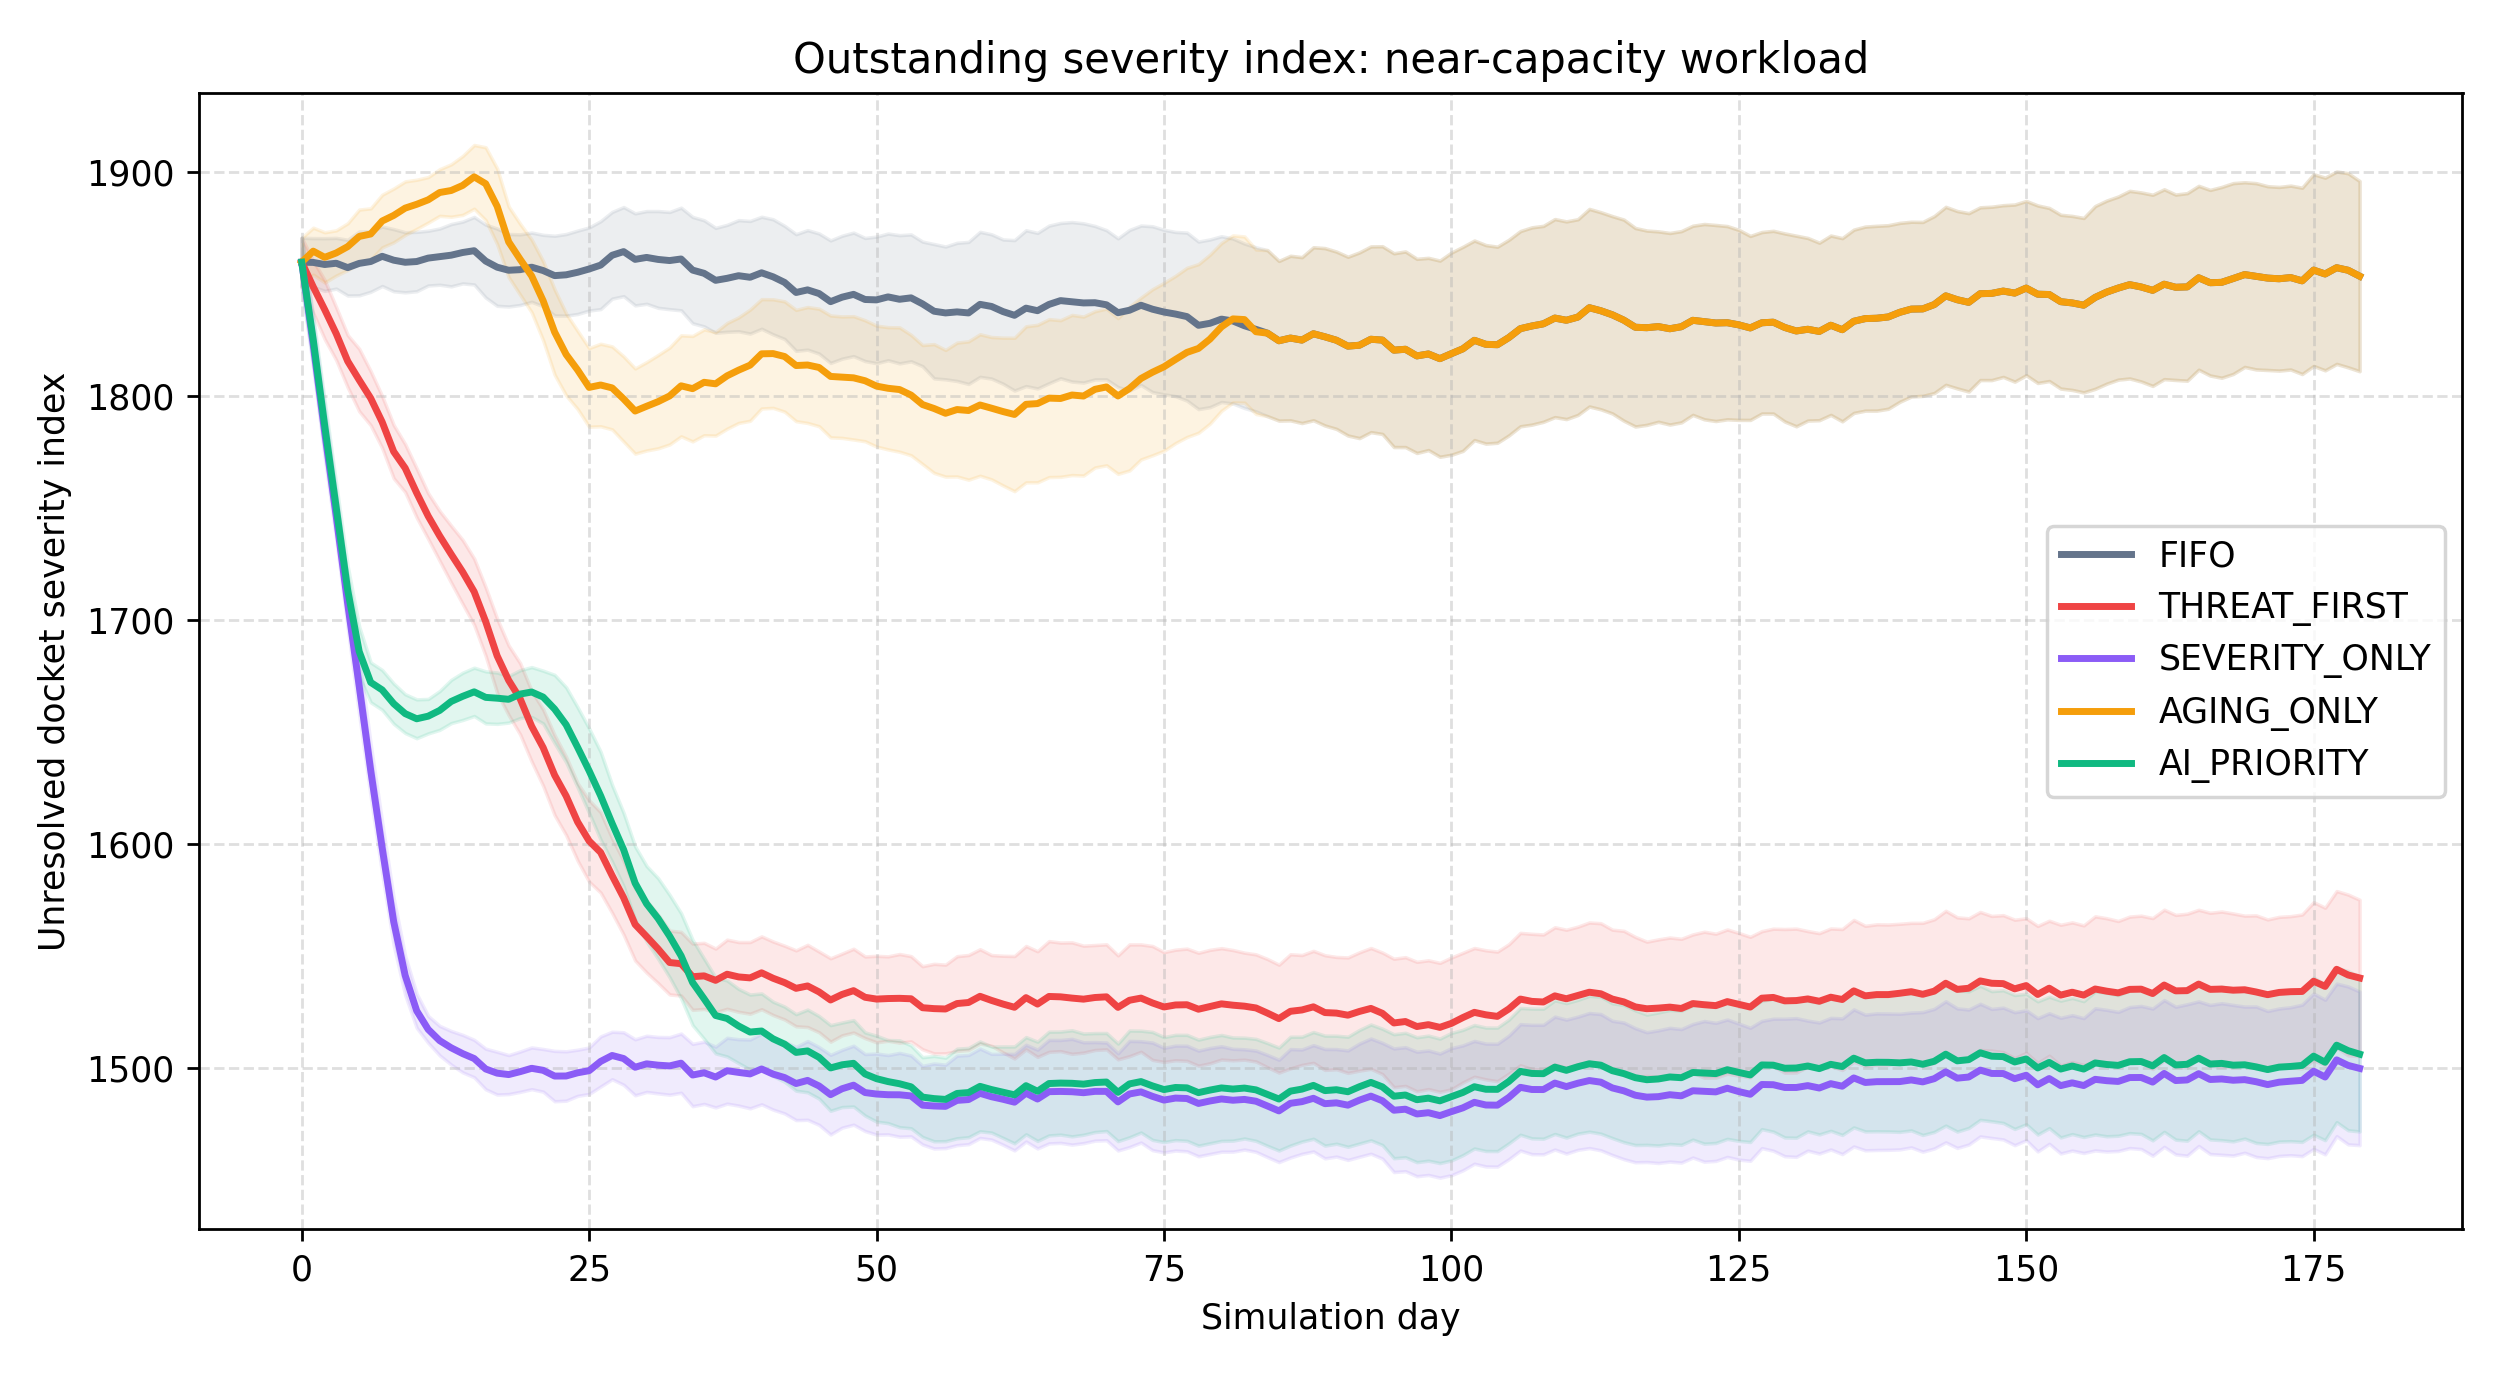
\includegraphics[width=\linewidth]{../evaluation/plots/simulation_backlog_severity_decay.png}
\caption{Cumulative Docket Backlog Severity Decay over 180 Court Days.}
\label{fig:decay}
\end{figure}

\subsection{Semantic Retrieval \& BNS Translation}
In Table~\ref{tab:retrieval_benchmark}, we evaluated retrieval performance across canonical Indian legal queries. Traditional BM25 exhibited an overlap of only 1.64 / 10 with Legal-BERT. Crucially, on modern BNS queries (e.g., Section 103 BNS), BM25 produced 0\% recall on historical IPC precedents, whereas our hybrid pipeline achieved accurate cross-regime precedent discovery.

\begin{table}[h]
\centering
\caption{Retrieval Model Overlap and Cross-Regime Match}
\label{tab:retrieval_benchmark}
\small
\begin{tabular}{llcc}
\toprule
Query Domain & Example Section & BM25-BERT Overlap & Cross-Regime \\
\midrule
Statutory IPC & Murder (IPC 302) & 3 / 10 & N/A \\
Statutory IPC & Rape (IPC 376) & 0 / 10 & N/A \\
Cross-Regime BNS & Murder (BNS 103) & 0 / 10 & \textbf{YES} \\
Cross-Regime BNS & Rape (BNS 64) & 1 / 10 & \textbf{PARTIAL} \\
\bottomrule
\end{tabular}
\end{table}

\subsection{Summarization Quality}
Evaluating Gemini 2.5 Flash summaries against source judgments yielded a ROUGE-1 precision of 0.8650, ROUGE-L of 0.4107, and a statutory section preservation rate of 100.0\% at a 17.4\% compression ratio.

\subsection{Global Explainability (TreeSHAP)}
Feature attribution analysis across 863 cases (Figure~\ref{fig:shap}) shows that the learned model relies most on the immediate-threat flag ($\text{mean absolute SHAP} = 1.188$), followed by offence severity ($0.395$). Since the training targets are generated from a formula that uses these features, these attributions describe reproduction of that formula; they do not independently validate legal priority.

\begin{figure}[h]
\centering
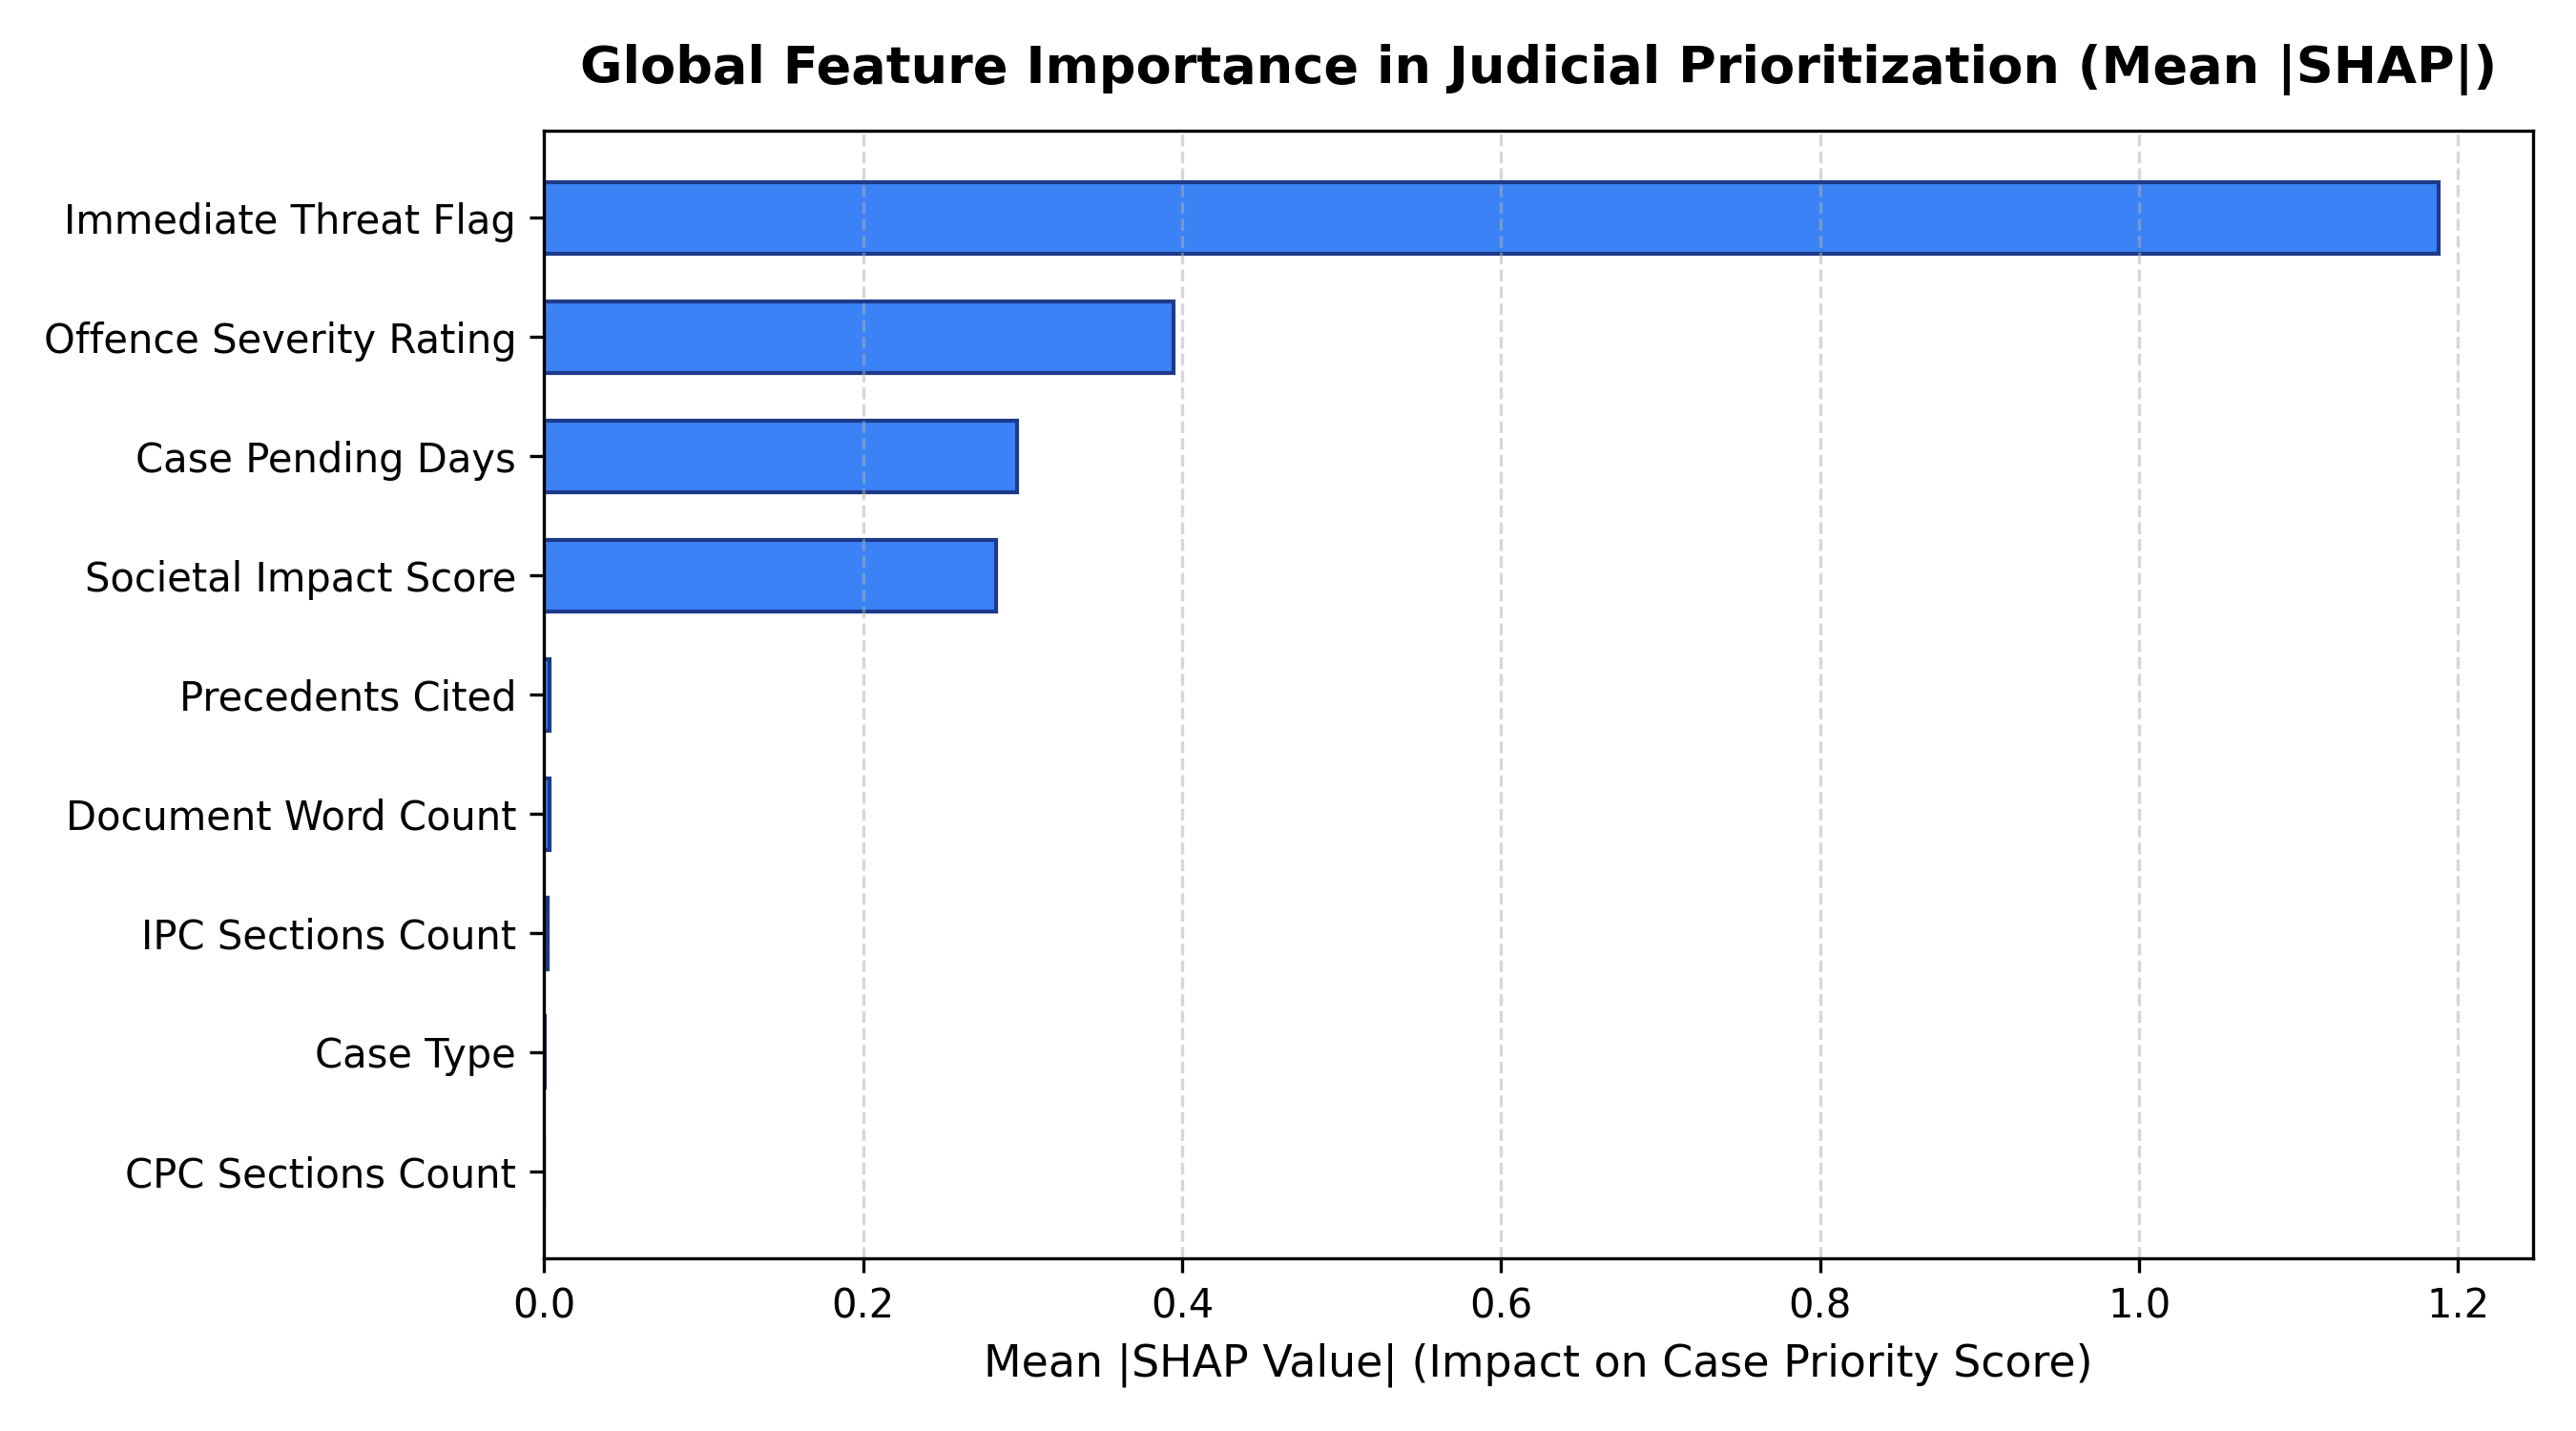
\includegraphics[width=\linewidth]{../evaluation/plots/shap_feature_importance.png}
\caption{Global Feature Importance Derived via TreeSHAP.}
\label{fig:shap}
\end{figure}

\subsection{Priority-Score Validation Limits}
The priority model is evaluated as an approximation of programmatically generated labels, not against independent lawyer judgments. Correlation between severity and priority is not independent validation because severity contributes directly to the label formula. Lawyer-adjudicated urgency labels on a held-out set are required before claiming legal validity or expert agreement.

\section{Conclusion}
We presented an end-to-end multi-agent AI system for judicial decision support. By combining cross-regime penal translation, explainable scheduling, and discrete-event simulation, this work illustrates how scheduling policies can change simulated waiting-time trade-offs under explicit assumptions. The simulation does not establish real-world reductions in pendency or fairness; validating those outcomes requires lawyer-reviewed urgency labels and registry filing, listing, and capacity data.

\bibliographystyle{ACM-Reference-Format}
\begin{thebibliography}{9}
\bibitem{chalkidis2020legalbert}
Ilias Chalkidis et al. 2020. LEGAL-BERT: The Muppets straight out of Law School. In \textit{Findings of EMNLP 2020}.
\bibitem{lundberg2017unified}
Scott M. Lundberg and Su-In Lee. 2017. A Unified Approach to Interpreting Model Predictions. In \textit{NeurIPS 2017}.
\end{thebibliography}

\end{document}
